%!TEX program = xelatex

\documentclass{progartcn}
\usepackage{graphicx}
\usepackage[dvipsnames]{xcolor}
\usepackage{wrapfig}
\usepackage{enumerate}
\usepackage{amsmath,mathrsfs,amsfonts}
\usepackage{booktabs}
\usepackage{tabularx}
\usepackage{colortbl}
\usepackage{multirow,makecell}
\usepackage{multicol}
\usepackage{ulem} % \uline
\usepackage{listings}
\usepackage{tikz}
\usepackage{tcolorbox}
\usepackage{fontawesome}


\title{\bfseries\sffamily
  计算机系统结构实验6 \\ 简单的类 MIPS 多周期流水化处理器实现
}
\author{胡晨志 521021910107}
\date{}


\begin{document}

\sloppy % 解决中英文混排文字超出边界问题


\maketitle
\thispagestyle{empty}

\begin{abstract}
\noindent 在lab06中,在lab基础上设计简单的流水线 CPU。通过本次实验,可以更加熟悉 Verilog 模块化编程,并加深对流水线和 hazard 的认识和理解。

\vspace{2ex}
\noindent \textbf{关键字:}Vivado,\hspace{.5em}Verilog
\end{abstract}

%\tableofcontents

%\setcounter{page}{0}
%\newpage

\section{实验目的}

理解 CPU Pipeline、流水线冒险及相关性,在lab5基础上设计简单流水线CPU

\section{原理分析}

本次实验中我完成了\verb|lw|,\verb|sw|,\verb|beq|,\verb|bne|,\verb|add|,\verb|sub|,\verb|and|,\verb|or|,\verb|slt|,\verb|j|,\verb|sll|,\verb|srl|,\verb|jr|等13条指令。

本次实验的主要难点在于 fowarding。上述指令中\verb|beq|,\verb|bne|,\verb|jr|和其余R型指令均需要用到 fowarding。在实现过程中,先得到 fowarding 的条件,通过条件判断是否 foward。实现时须注意 foward 的优先级,越早的阶段优先级越高。

\section{功能实现}

这里主要介绍顶层模块的设计。

\subsection{常用管线}

首先是各个流水线寄存器所用到的管线和其他常用管线的定义,如 </>CODE \ref{cd:1} 所示。

\begin{lstlisting}[language=verilog,caption={常用管线.v},label={cd:1}]
    // Pipeline stage registers
    // IF/ID
    wire [31:0] IFID_pcPlus4, IFID_instr;
    wire [4:0] IFID_INSTRS = IFID_instr[25:21], IFID_INSTRT = IFID_instr[20:16],
         IFID_INSTRD = IFID_instr[15:11];
    wire BRANCH;
    wire JUMP;
    wire JUMP_REGISTER;
    
    // ID/EX
    wire [31:0] IDEX_readData1, IDEX_readData2, IDEX_immSext;
    wire [4:0] IDEX_instrRs, IDEX_instrRt, IDEX_instrRd;
    wire [8:0] IDEX_ctrl;
    wire [1:0] IDEX_ALUOP = IDEX_ctrl[7:6];
    wire IDEX_REGDST = IDEX_ctrl[8], IDEX_ALUSRC= IDEX_ctrl[5], 
        IDEX_BRANCH = IDEX_ctrl[4], IDEX_MEMREAD = IDEX_ctrl[3], 
        IDEX_MEMWRITE = IDEX_ctrl[2], IDEX_REGWRITE = IDEX_ctrl[1],
        IDEX_MEMTOREG = IDEX_ctrl[0];
        
    wire [4:0] DST_REG;
    wire [31:0] ALU_RES;
        
    // EX/EM
    wire [31:0] EXMEM_aluRes, EXMEM_writeData;
    wire [4:0] EXMEM_dstReg;
    wire [4:0] EXMEM_ctrl;
    wire EXMEM_zero;
    wire EXMEM_BRANCH = EXMEM_ctrl[4], EXMEM_MEMREAD = EXMEM_ctrl[3],
        EXMEM_MEMWRITE = EXMEM_ctrl[2], EXMEM_REGWRITE = EXMEM_ctrl[1],
        EXMEM_MEMTOREG = EXMEM_ctrl[0];
        
    // MEM/WB
    wire [31:0] MEMWB_readData, MEMWB_aluRes;
    wire [4:0] MEMWB_dstReg;
    wire [1:0] MEMWB_ctrl;
    wire MEMWB_REGWRITE = MEMWB_ctrl[1], MEMWB_MEMTOREG = MEMWB_ctrl[0];
\end{lstlisting}

\subsection{取址阶段}

取址阶段,PC 在时钟上升沿更新的。由于插入停顿时程序不能向前执行,所以 PC 和 IF/ID 流水线寄存器此时不能更新。同时,为了解决控制冒险,在出现条件跳转时,需要将之前取出的指令清除(flush)。分支和跳转的条件将会在之后介绍。该阶段顶层模块如 </>CODE \ref{cd:2} 所示,PC 和 IF/ID 寄存器如 </>CODE \ref{cd:2} 和 </>CODE \ref{cd:3} 所示。 

\begin{lstlisting}[language=verilog,caption={取址阶段},label={cd:2}]
    // Instruction Fetch Stage
    wire [31:0] PC;
    wire [31:0] PC_PLUS_4, BRANCH_ADDR, JR_DST, SELECT_PC_A, SELECT_PC_B, NEXT_PC, IF_INSTR;
    assign JUMP = IF_INSTR[31:26] == 6'b000010 ? 1 : 0;
    assign PC_PLUS_4 = PC + 4;
    
    MUX_32bits selectPCMux_A(.Input2(PC_PLUS_4), .Input1({PC_PLUS_4[31:28], IF_INSTR[26:0], 2'b00}),
        .Out(SELECT_PC_A), .sel(JUMP));
    MUX_32bits selectPCMux_B(.Input2(SELECT_PC_A), .Input1(JR_DST),
        .Out(SELECT_PC_B), .sel(JUMP_REGISTER));
    MUX_32bits nextPCMux(.Input2(SELECT_PC_B), .Input1(BRANCH_ADDR), .Out(NEXT_PC),
        .sel(BRANCH));
    InstMemory instrMem(.ReadAddress(PC), .Instruction(IF_INSTR));
    
    PC mainPC(.Clk(clk), .reset(reset), .STALL(STALL), .NEXT_PC(NEXT_PC), .PC(PC));
    
    buffer1 IFID(.Clk(clk), .stall(STALL), .branch(BRANCH), .PC_PLUS_4(PC_PLUS_4),
        .IF_INSTR(IF_INSTR), .IFID_instr(IFID_instr), .IFID_pcPlus4(IFID_pcPlus4));
\end{lstlisting}

\begin{lstlisting}[language=verilog,caption={PC.v},label={cd:3}]
`timescale 1ns / 1ps
module PC(
    input Clk,
    input reset,
    input STALL,
    input [31:0] NEXT_PC,
    output [31:0] PC
    );
    reg [31:0] pc;

    initial begin
        pc = 0;
    end 

    always @ (reset)
        pc = 0;

    always @(posedge Clk)
    if(!STALL)
        begin
            pc <= NEXT_PC;
        end
    assign PC = pc;
endmodule
\end{lstlisting}

\begin{lstlisting}[language=verilog,caption={buffer1.v},label={cd:4}]
`timescale 1ns / 1ps
module buffer1(
    input Clk,
    input reset,
    input stall,
    input branch,
    input [31:0] PC_PLUS_4,
    input [31:0] IF_INSTR,
    output [31:0] IFID_instr, IFID_pcPlus4
    );
    reg [31:0] pcPlus4;
    reg [63:32] instr;

    always @(reset)
    begin
        pcPlus4 = 0;
        instr = 0;
    end

    always @(posedge Clk)
    begin
        if (!stall)
        begin
            pcPlus4 <= PC_PLUS_4;
            instr <= IF_INSTR;
        end
        if (branch)
            instr <= 0;
    end
    
    assign IFID_instr = instr, IFID_pcPlus4 = pcPlus4;
endmodule
\end{lstlisting}

\subsection{译码阶段}

这里的实现中,将跳转的判定和跳转地址的计算移到了译码阶段,只要寄存器读出的数据相等就可以跳转。这是为了减少对流水线寄存器清除的次数,提高执行效率,同时也也有利于简化流水线。

需要注意分支指令和寄存器跳转指令可能产生数据冒险,故此处加入了 fowarding。译码阶段顶层模块代码如 </>CODE \ref{cd:4} 所示。buffer2 的实现与 buffer1 类似,这里不作赘述。

\begin{lstlisting}[language=verilog,caption={译码阶段},label={cd:5}]
    // Decode Stage
    wire [8:0] CTRL_OUT;
    Ctr mainCtr(.OpCode(IFID_instr[31:26]), .RegDst(CTRL_OUT[8]), 
        .ALUOp(CTRL_OUT[7:6]), .ALUSrc(CTRL_OUT[5]), .Branch(CTRL_OUT[4]),
        .MemRead(CTRL_OUT[3]), .MemWrite(CTRL_OUT[2]), .RegWrite(CTRL_OUT[1]),
        .MemToReg(CTRL_OUT[0]));
    
    wire [31:0] READ_DATA_1, READ_DATA_2, REG_WRITE_DATA;
    Registers regs(.Clk(clk), .readReg1(IFID_INSTRS), .readReg2(IFID_INSTRT), 
        .writeReg(MEMWB_dstReg), .writeData(REG_WRITE_DATA), 
        .regWrite(MEMWB_REGWRITE), .reset(reset), .readData1(READ_DATA_1), 
        .readData2(READ_DATA_2));
    
    wire [31:0] IMM_SEXT;
    signext sext(.inst(IFID_instr[15:0]), .out(IMM_SEXT));
    wire [31:0] IMM_SEXT_SHIFT = IMM_SEXT << 2;
    
    wire BRANCH_FWD_ID_A =
        IDEX_ctrl[1] & DST_REG != 0 & DST_REG == IFID_INSTRS;
    wire BRANCH_FWD_ID_B =
        IDEX_ctrl[1] & DST_REG != 0 & DST_REG == IFID_INSTRT;
    wire BRANCH_FWD_EX_A = 
        EXMEM_REGWRITE & EXMEM_dstReg != 0 & EXMEM_dstReg == IFID_INSTRS;
    wire BRANCH_FWD_EX_B = 
        EXMEM_REGWRITE & EXMEM_dstReg != 0 & EXMEM_dstReg == IFID_INSTRT;
    wire BRANCH_FWD_MEM_A = 
        MEMWB_REGWRITE & MEMWB_dstReg != 0 & 
        !(EXMEM_REGWRITE & EXMEM_dstReg != 0 & EXMEM_dstReg != IFID_INSTRS) &
        MEMWB_dstReg == IFID_INSTRS;
    wire BRANCH_FWD_MEM_B = 
        MEMWB_REGWRITE & MEMWB_dstReg != 0 & 
        !(EXMEM_REGWRITE & EXMEM_dstReg != 0 & EXMEM_dstReg != IFID_INSTRT) &
        MEMWB_dstReg == IFID_INSTRT;
        
    wire [31:0] BRANCH_SRC_A = BRANCH_FWD_ID_A ? ALU_RES : BRANCH_FWD_EX_A ? EXMEM_aluRes : 
        BRANCH_FWD_MEM_A ? REG_WRITE_DATA : READ_DATA_1;

    wire [31:0] BRANCH_SRC_B = BRANCH_FWD_ID_B ? ALU_RES : BRANCH_FWD_EX_B ? EXMEM_aluRes : 
        BRANCH_FWD_MEM_B ? REG_WRITE_DATA : READ_DATA_2;
    
    assign BRANCH_ADDR = IMM_SEXT_SHIFT + IFID_pcPlus4;
    assign BRANCH = CTRL_OUT[4] ? (!IFID_instr[26] && BRANCH_SRC_A == BRANCH_SRC_B )
        || (IFID_instr[26] && BRANCH_SRC_A != BRANCH_SRC_B ) : 0;
    assign JUMP_REGISTER = CTRL_OUT[8] && IMM_SEXT[5:0]==6'b001000;
    assign JR_DST = BRANCH_SRC_A;
    
    buffer2 IDEX(.Clk(clk), .reset(reset), .STALL(STALL), .CTRL_OUT(CTRL_OUT),
        .READ_DATA_1(READ_DATA_1), .READ_DATA_2(READ_DATA_2), .IMM_SEXT(IMM_SEXT),
        .IFID_INSTRS(IFID_INSTRS), .IFID_INSTRT(IFID_INSTRT), .IFID_INSTRD(IFID_INSTRD),
        .IDEX_readData1(IDEX_readData1), .IDEX_readData2(IDEX_readData2), .IDEX_immSext(IDEX_immSext),
        .IDEX_instrRs(IDEX_instrRs), .IDEX_instrRt(IDEX_instrRt), .IDEX_instrRd(IDEX_instrRd),
        .IDEX_ctrl(IDEX_ctrl));
\end{lstlisting}

\subsection{执行阶段}

由于可能用到寄存器的值,故需要加入 fowarding 来避免数据冒险。其余部分除了更新流水线寄存器之外,和单周期处理器几乎相同,如 </>CODE \ref{cd:6} 所示。

\begin{lstlisting}[language=verilog,caption={执行阶段},label={cd:6}]
    // Forwarding Unit
    wire FWD_EX_A = 
        EXMEM_REGWRITE & EXMEM_dstReg != 0 & EXMEM_dstReg == IDEX_instrRs;
    wire FWD_EX_B = 
        EXMEM_REGWRITE & EXMEM_dstReg != 0 & EXMEM_dstReg == IDEX_instrRt;
    wire FWD_MEM_A = 
        MEMWB_REGWRITE & MEMWB_dstReg != 0 & 
        !(EXMEM_REGWRITE & EXMEM_dstReg != 0 & EXMEM_dstReg != IDEX_instrRs) &
        MEMWB_dstReg == IDEX_instrRs;
    wire FWD_MEM_B = 
        MEMWB_REGWRITE & MEMWB_dstReg != 0 & 
        !(EXMEM_REGWRITE & EXMEM_dstReg != 0 & EXMEM_dstReg != IDEX_instrRt) &
        MEMWB_dstReg == IDEX_instrRt;
        
    // Execution Stage
    wire [31:0] ALU_SRC_A = FWD_EX_A ? EXMEM_aluRes : 
        FWD_MEM_A ? REG_WRITE_DATA : IDEX_readData1;
    wire [31:0] ALU_SRC_B = IDEX_ALUSRC ? IDEX_immSext : FWD_EX_B ? EXMEM_aluRes :
        FWD_EX_B ? EXMEM_aluRes : FWD_MEM_B ? REG_WRITE_DATA : IDEX_readData2;
    wire [31:0] MEM_WRITE_DATA = FWD_EX_B ? EXMEM_aluRes :
        FWD_EX_B ? EXMEM_aluRes : FWD_MEM_B ? REG_WRITE_DATA : IDEX_readData2;
         
    wire [3:0] ALU_CTRL_OUT;
    ALUCtr aluCtr(.Funct(IDEX_immSext[5:0]), .ALUOp(IDEX_ALUOP), 
        .ALUCtrOut(ALU_CTRL_OUT));
    
    wire ZERO;
    ALU alu(.Input1(ALU_SRC_A), .Input2(ALU_SRC_B), .Input3(IDEX_immSext[10:6]), .ALUCtr(ALU_CTRL_OUT), .Zero(ZERO),
        .ALURes(ALU_RES));
        
    MUX_5bits dstRegMux(.Input2(IDEX_instrRt), .Input1(IDEX_instrRd), .sel(IDEX_REGDST),
        .Out(DST_REG));
    
    buffer3 EXMEM(.Clk(clk), .reset(reset), .IDEX_ctrl(IDEX_ctrl), .ZERO(ZERO),
        .ALU_RES(ALU_RES), .MEM_WRITE_DATA(MEM_WRITE_DATA), .DST_REG(DST_REG),
        .EXMEM_aluRes(EXMEM_aluRes), .EXMEM_writeData(EXMEM_writeData),
        .EXMEM_ctrl(EXMEM_ctrl), .EXMEM_zero(EXMEM_zero), .EXMEM_dstReg(EXMEM_dstReg));
\end{lstlisting}

\subsection{访存和写回}

除了更新流水线寄存器之外,和单周期处理器几乎相同,如 </>CODE \ref{cd:7} 所示。

\begin{lstlisting}[language=verilog,caption={访存和写回},label={cd:7}]
    // Memory Stage
    wire [31:0] MEM_READ_DATA;
    dataMemory dataMem(.Clk(clk), .address(EXMEM_aluRes), 
        .writeData(EXMEM_writeData), .memRead(EXMEM_MEMREAD), 
        .memWrite(EXMEM_MEMWRITE), .readData(MEM_READ_DATA));

    buffer4 MEMWB(.Clk(clk), .reset(reset), .EXMEM_ctrl(EXMEM_ctrl[1:0]),
        .MEM_READ_DATA(MEM_READ_DATA), .EXMEM_aluRes(EXMEM_aluRes), .EXMEM_dstReg(EXMEM_dstReg),
        .MEMWB_readData(MEMWB_readData), .MEMWB_aluRes(MEMWB_aluRes), .MEMWB_dstReg(MEMWB_dstReg), .MEMWB_ctrl(MEMWB_ctrl));
    
    // Write Back Stage
    MUX_32bits writeDataMux(.Input1(MEMWB_readData), .Input2(MEMWB_aluRes), 
        .sel(MEMWB_MEMTOREG), .Out(REG_WRITE_DATA));
\end{lstlisting}

\subsection{插入停顿}

只有一种情况需要插入停顿,即在\verb|lw|指令后的一条指令直接访问\verb|lw|所加载的寄存器的数据。由于此时数据还在数据存储器内,所以无法通过转发解决数据冒险,只能暂停流水线。代码如 </>CODE \ref{cd:8} 所示。

\begin{lstlisting}[language=verilog,caption={插入停顿},label={cd:8}]
// Hazard detection
    wire STALL = IDEX_MEMREAD & 
        (IDEX_instrRt == IFID_INSTRS | IDEX_instrRt == IFID_INSTRT);
\end{lstlisting}

\section{结果验证}

\subsection{测试用激励文件}

\verb|Top_tb.v|如</>CODE \ref{cd:7}所示。这里采用与 lab05 相同的测试集。

\begin{lstlisting}[language=verilog,caption={Top\_tb.v},label={cd:8}]
`timescale 1ns / 1ps

module Top_tb(

    );
    reg clk, reset;
    always #5 clk = !clk;
    
    Top top(.clk(clk), .reset(reset));
    
    initial begin
        $readmemb("Instruction", top.instrMem.InstMemFile);
        $readmemh("Data", top.dataMem.memFile);
        clk = 1;
        reset = 1;
        #25 reset = 0;
    end
endmodule
\end{lstlisting}

\subsection{仿真测试}

仿真结果如图\ref{fig:1}所示。可以看到8号寄存器的最终数值为117,说明运行结果正确。

\begin{figure}[htbp]
    %是可选项 h表示的是here在这里插入,t表示的是在页面的顶部插入
    \centering
    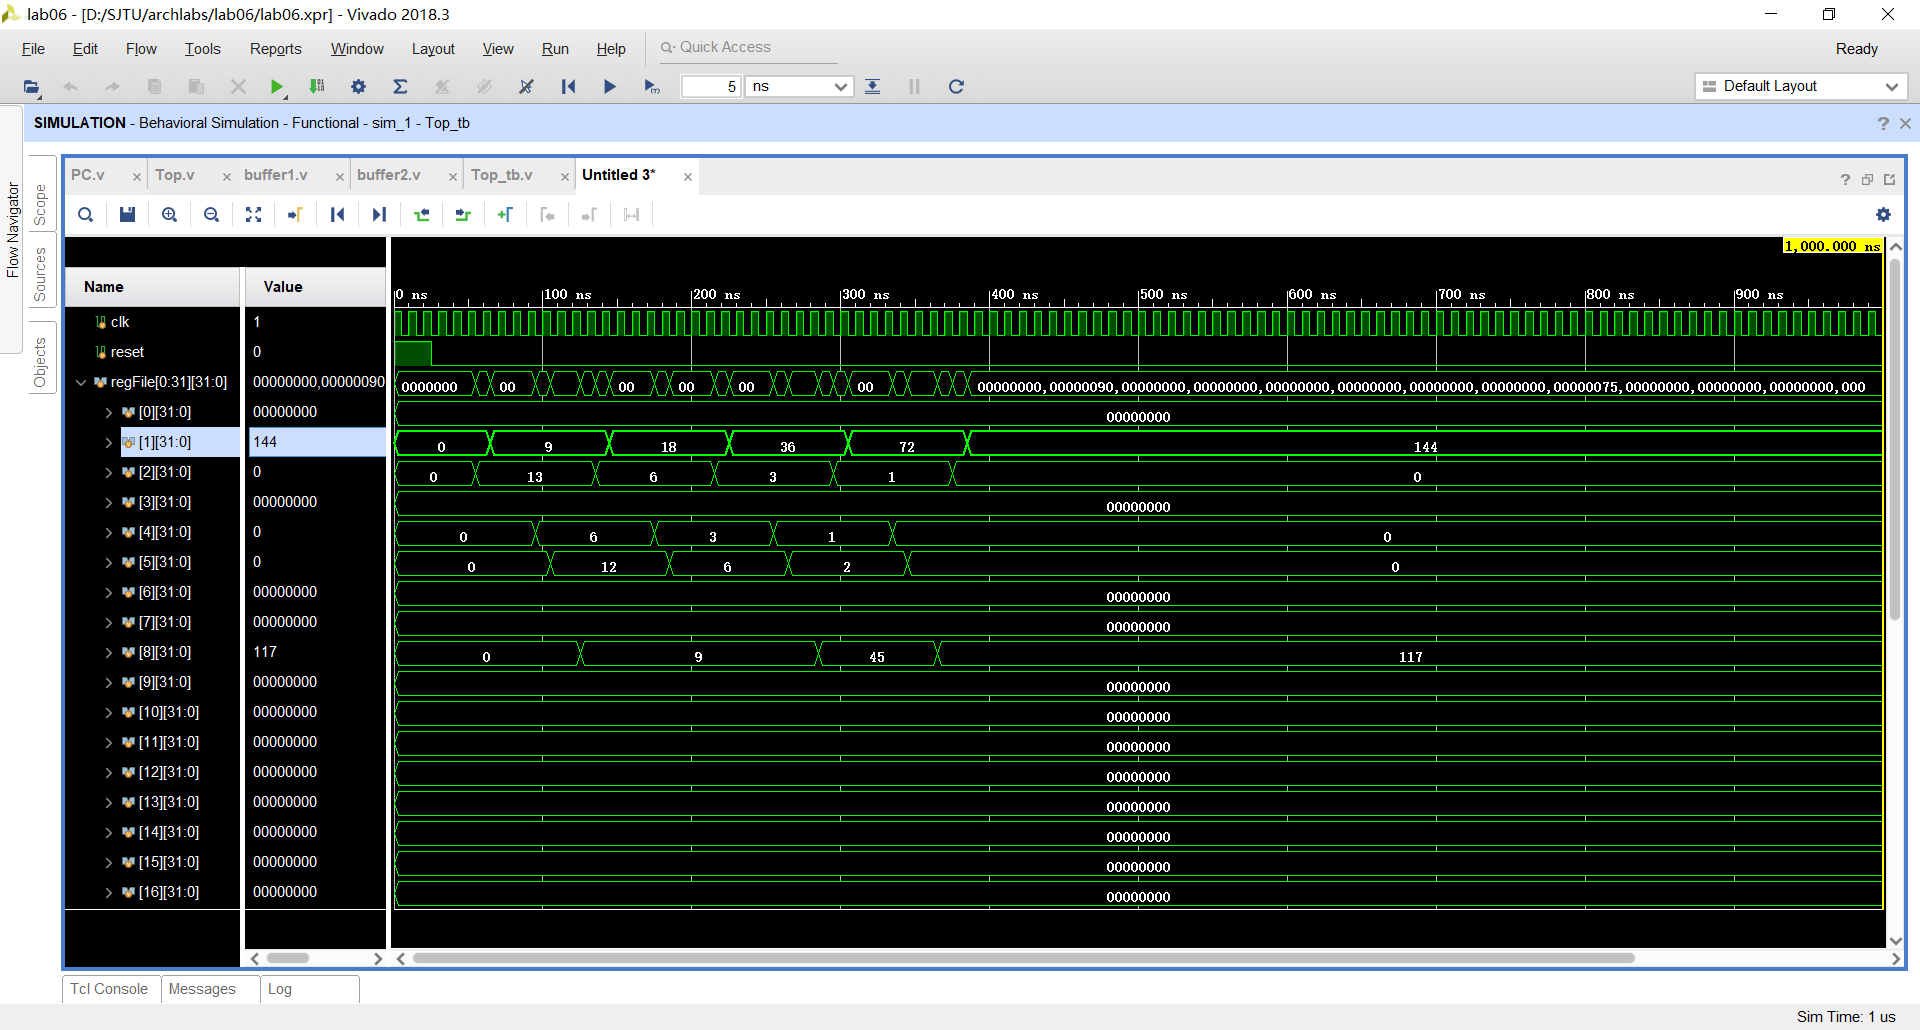
\includegraphics[scale=0.3]{../figure/06/lab06-1.PNG}
    \caption{数据存储器实验结果}\label{fig:1}
\end{figure}

\section{反思与总结}

本次实验实现了流水线,总体而言相当有挑战性的。由于实验中用到了大量的管线,为管线设计一套命名规范显得至关重要。此外,在许多细节方面也要考虑,比如 fowarding 的优先级,以及分支指令和跳转指令的优先级。这些在理论课上都是很难体会到的,只有真正上手实践才能有深刻的感受。

\end{document}
